\section{Эксперимент}
\label{sec:Chapter5} \index{Chapter5}

\subsection{Описание эксперимента}

Постановка эксперимента. Что планируется сделать и какие результаты хочется получить. Какие метрики будем использовать и по каким метрикам будем сравнивать.

\subsubsection*{Выбор модели для эксперимента}

В рамках поставленного эксперимента поставлена задачи исследования работы алгоритма PUL для задачи распознавания ключевых точек для нескольких моделей:
\begin{enumerate}
\item HRNet
\item ViTPose
\item RTMPose ???
\item SimCC + ResNet ???
\end{enumerate}

Предложенные модели будут обучены на исходном датасете в течение 20 эпох. Таким образом будут получены базовые наборы весов, от которых и будет дпроводиться дальнейшее исследование.

\subsubsection*{Описание метода доменной адаптации}
Отбор точек будет произвед путем сравнения ЗНАЧЕНИЯ (ЗАМЕНИТЬ) с заранее заданным пороговым значением. ЗНАЧЕНИЕ будет отбираться двумя способами:
\begin{enumerate}
\item Средняя уверенность в предсказанных значениях\\
Для каждго предсказанного результата модель возвращает значение уверенности в своем предсказании. Усредняя это значении по всем ключевым точкам получаем среднюю уверенность для фотографии
\item Средняя уверенность для всех видимых точек\\
Так как увереннсть на точках, которые не видно на фотографии может сильно занижать среднее ЗНАЧЕНИЕ для всего результата, то принято решение отбрасывать эти значения при высчитываании ЗНАЧЕНИЯ
\end{enumerate}

По порогу уверенности будет отбираться набор значений с псевдоразметкой, на которой модель будет дообучаться. Таким образом будет проведено N (УКАЗАТЬ ТОЧНОЕ ЗНАЧЕНИЕ) итераций адаптации и сравнено значение результатов модели при различных способах отбора псевдоразметки. Также в рамках эксперимента произведено полное дообучение модели на размеченном целевом домене и результаты буду предоставлен для сравнения с адаптированными.

\subsubsection*{Метрики оценки качества распознавания}

ТАКЖЕ НЕОБХОДИМО СКАЗАТЬ ОБ МЕТРИКАХ ОЦЕНКИ РАСПОЗНАВАНИЯ

Для проведения количественного анализа результатов эксперимента, необходимо выделить несколько метрик, с помощью которых можно будет отобрать наилучшие результаты.

PCK

ФОРМУЛА И ОБЪЯСНЕНИЕ

OKS

ФОРМУЛА И ОБЪЯСНЕНИЕ

AP/mAP

ФОРМУЛА И ОБЪЯСНЕНИЕ

\subsubsection*{Используемые ресурсы}

ТАКЖЕ НЕОБХОДИМО СКАЗАТЬ ОБ ИСПОЛЬЗУЕМЫХ РЕСУРСАХ


\subsection{Данные}

По условиям задачи доменной адаптации необходимо найти два набора данных для эксперимента. Далее приведем информацию о выбранных доменах и их характеристиках.

\subsubsection*{Исходные домен}

%Здесь надо рассказать про датасет коко и привести немного сведений о нем.\\
%Пример ФОТОграфий из датасета.\\
%Рассказать про аннотацию тут.\\
%Рассказать про отбор фотографий из-за граниченности ресурсов.

В качестве исходного домена выбран набор данных Common Objects in Context \cite{COCO_dataset}. COCO — это крупный датасет, широко используемый в области компьютерного зрения для задач распознавания объектов, сегментации, и создания описательных подписей к изображениям. Он был создан Microsoft и с тех пор стал стандартом для обучения и оценки алгоритмов компьютерного зрения.

\begin{figure}[h]
	\centering
	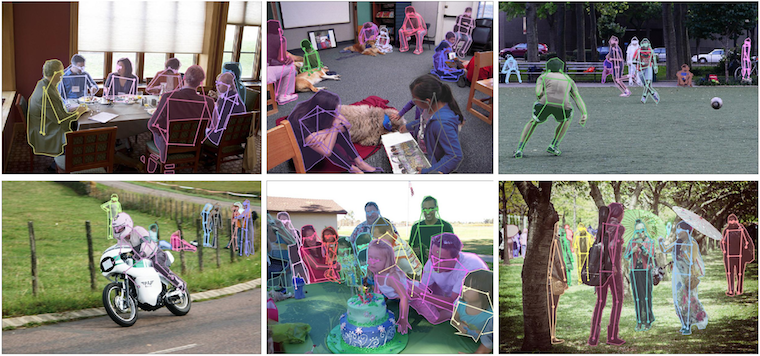
\includegraphics[width=\textwidth]{./images/coco_dataset.png}
	\caption{Примеры изображений из набора данных COCO. \cite{COCO_topology}}
	\label{fig:coco_dataset}
\end{figure}

Учитывая, что в рамках соревнований COCO была и задача детекции ключевых точек (Keypoint detection) \cite{COCO_topology}, то часть этого набора данных была размечена под нее. Если быть точным, то датасет включает более 250 тысяч аннотаций людей на различных изображениях. Формат аннотаций включает в себя:

\begin{enumerate}

\item \textit{id} - уникальный номер аннотации;

\item \textit{image\_id} - уникальный номер изображения, которому принадлежит данная аннотация;

\item \textit{category\_id} - уникальный номер категории, к которой относится данная аннотация. Для задачи оценки позы везде выставляется категория person;

\item \textit{keypoints} - массив из 17 ключевых точек, для каждой их которых указаны координа (x, y) на изобраении, а также информация о видимости. Точки, которые не представлены на изображении заполняются нулями;

\item \textit{num\_keypoints} - здесь содержится информация о количестве размеченных точек для данной аннотации;

\item \textit{bbox} - информация об обграничивающем человека прямоугольнике. Значения внутри лежат в следующем формате: $[x, y, width, height]$;

\item \textit{area} площадь сегментированного человека. Значение необходимо при высчитывании метрики OKS;

\item \textit{iscrowd} - информация о том, одиночный человек представлен на изображении или толпа людей.

\end{enumerate}

Также в рамках задачи Keypoint Detection была введена метрика OKS и метрика mAP, о которых было рассказано ранее. Они представляют собой единые критерии для оценки моделей, что облегчает сравнение и улучшение результатов различных алгоритмов, поэтому регулярно используются для оценки  новых методов и технологий.

В рамках задачи были выбраны 8000 аннотаций, которые содержат все 17 ключевых точек то топологии COCO. На них и было произведено обучение моделей для получения бейзлайнов эксперимента.

\subsubsection*{Целевой домен}

%Описание собранных данных. Численный объем датасета. Возможно количество локаций и распределение по ним.

%Необходимо предоставить данные по распределению данных между людьми, по количеству данных для обучения/тестирования. Предоставить данные по локациям. Предоставить картинки с примерами данных, которые были собраны.

%Описание системы полуавтоматической разметки данных. Что там использовалось и как проходит разметка.

В качестве целевого набора данных был собран отдельный набор данных боксеров. В наборе данных представлены 2 человека, снятые с 3 ракурсов: профиль, анфас и 3/4. Датасет состоит из 10 видеозаписей, которые содержат порядка 10 тысяч кадров. Для проведения эксперимента выбрано 2,6 тысячи изображений, которые были впоследствие размечены. Из них для тестовой выборки отобрано около 420 изображений, а оставшиеся 2200 составили обучающую выборку, на которой и проводилась адаптация.

ПРИМЕРЫ ИЗОБРАЖЕНИЙ

В рамках задачи по аннотированию собранных данных была разработана система полуавтоматической разметки изображений pose-markup \cite{pose_markup}. Она представляет собой предобученную модель распознавания ключевых точек и инструмент для визуальной корректировки данных экспертом.

Для автоматической части использовалась модель BlazePose от проекта MediaPipe \cite{mediapipe}. Выбор сделан благодаря высоким характеристикам скорости инференса результатов и их точности у данного решения. А также для того, чтобы избежать корреляции размеченных данных с предсказаниями, которые будут оцениваться в рамках эксперимента. Результат, возвращаемый моделью был преобразован к формату аннотаций COCO, который был описан выше и сохранен в формате JSON. 

Как можно видеть на ИЗОБРАЖЕНИИ, модель имеет неточности, которые необходимо было исправить эксперту. Для этой цели использовалась вторая часть программы - инструмент для визуальной корректировки данных экспертом. В ТАБЛИЦЕ  предоставлена сводная информация о количестве изменений, внесенных экспертом, а на ИЗОБРАЖЕНИИ представлена тепловая карта ключевых точек топологии, которые нуждались в корректировке. 



\subsection{Результаты эксперимента}

Предоставить относительно сухо результаты эксперимента. Можно дать базовый анализ ситуации и того, что мы видим.

Необходимо предоставить результаты по времени обучения нейросетей, времени дообучения нейросетей. \\ 
Собрать данные по количеству ошибок до-после обучения. Собрать данные по количеству ошибок при изменении домена. \\ 
Данные по ресурсам, на которых обучались нейросетки.


\newpage